\section{Experiment Design}
\label{sec:experiment}
In this section, we detail the overall experiment design and explain the reasoning behind specific experiment decisions.

\subsection{Experiment Protocol}
We recruited participants from a United States college town using various methods: online ads, digital bulletins, social media posts, physical flyers, and online newsletters. To ensure diversity, we prioritized non-students by placing physical flyers in public spaces like restaurants, cafes, and libraries beyond campus. As we monitored respondent demographics, we began selectively accepting non-student participants. If a respondent self-identified as a student, we thanked them and informed them of our current priority for non-students, though some self-identified students were still accepted. To prevent response bias, we framed the study as focusing on attitudes toward societal issues rather than measuring cognitive load and behaviors. The college Institutional Review Board reviewed and approved this study.

\begin{figure}[ht]
    \centering
    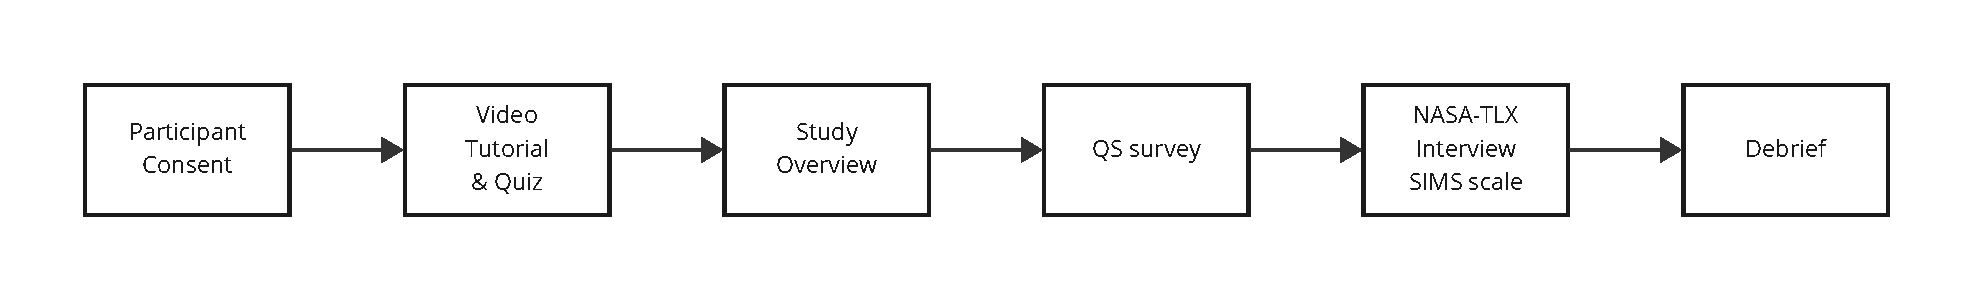
\includegraphics[width=1\textwidth]{content/image/study_flow.pdf}
    \caption{Study protocol}
    \label{fig:studyProtocol}
\end{figure}

Figure~\ref{fig:studyProtocol} visually represents the study protocol. Participants were invited to the lab to minimize external influences on cognitive load measurement and ensure consistency between sessions. The experiment involved participants using a 32-inch vertical monitor, ensuring all options on a QS were visible to minimize hidden information during decision-making. After consenting to the study, participants watched a pre-recorded video explaining the Quadratic mechanism and how QS operates without hints of interface operation. Participants then completed a short quiz to ensure their understanding of the QS mechanism. Those who failed to answer all questions correctly were asked to rewatch the video or consult the researcher until they could select the correct answers. The participant's screen was captured throughout the study. The researcher primed the participant that the study aimed to help local community organizers understand preferences on societal issues to better allocate resources. Participants were randomly assigned to one of four groups:

\begin{itemize}
    \item 6 options with a text-based interface
    \item 6 options with an interactive interface
    \item 24 options with a text-based interface
    \item 24 options with an interactive interface
\end{itemize}

Participants completed the survey independently, without the researcher's presence. Upon completion, they contacted the researcher. The researcher distributed the NASA-TLX cognitive load measurement and a short semi-structured interview about their experiences. This interview was audio recorded. The session concluded with a debriefing and a \$15 cash compensation. During the debriefing, participants were informed that the survey's true purpose was to measure cognitive load and interface design, and they could ask any questions.

\subsection{Experiment Design Choices}
This subsection details the justifications behind each experiment design decision. We made four major decisions:

\subsubsection{A between subject study}
We chose a between-subject study design for two main reasons. First, to minimize study fatigue given the complexity of responding to a QS survey, which could take up to 20 minutes. Conducting back-to-back experiments to measure cognitive load would be impractical, and asking participants to revisit the lab after several days would likely increase dropout rates and demotivate participants from attending in-person sessions. Second, we aimed to reduce the learning effect, which is challenging to eliminate, especially concerning interface operation and decision-making in the survey. Since preferences are constructed, we wanted to ensure that participants were not influenced by their previous preferences, which could affect their perceived cognitive load.

\subsubsection{Deciding number of survey options}
Ideally, understanding participants' cognitive load across multiple options would require enumerating all possible numbers of options to identify the "breaking point" where cognitive overload occurs. However, this approach is not feasible due to time and resource constraints. Therefore, we referred to prior literature to inform our choice of 6 and 24 options, representing short and long lists. Constant sum surveys and the Analytic Hierarchy Process (AHP) recommend fewer than ten and seven options, respectively~\cite{moroneyQuestionnaireDesignHow2019, saatyGroupDecisionMaking2013, saatyPrinciplesAnalyticHierarchy1987}. Some refer to the value $7$ based on human's cognitive processing capacity of $7\pm2$~\cite{millerMagicalNumberSeven1956} and a theoretical proof using the consistency ratio of a pairwise comparison metric~\cite{saaty2003magic}. A meta-analysis by~\textcite{chernevChoiceOverloadConceptual2015} surveyed 99 choice overload experiments and summarized that 6 and 24 are the modal values for short and long lists when testing choice overload. These two values were likely rooted in the original choice overload experiment\footnote{We believe that the original value decision was due to the limitations of the jam flavors.} by~\textcite{iyengarWhenChoiceDemotivating2000}. Thus, we adopted these values to align with established research.

\subsubsection{Context of the Study}
Participants completed a societal issue survey, following the methodology described by ~\textcite{chengCanShowWhat2021}. Surveying societal issues is relevant to every citizen, and easily conveys the concept of limited public sector resources that need prioritization across different areas. We curated a list of societal issues directly from the categories used by Charity Navigator~\cite{CharityNavigator2023}, a non-profit organization that evaluates over 20 thousand charities in the United States. Participants across all four groups were presented with options randomly drawn from 26 societal issues. The full list of these societal issues is provided in Appendix~\ref{sec:charityList}.

\subsubsection{Using NASA-TLX to measure cognitive load}
Several methods exist to measure cognitive load, including performance measures, psychophysiological measures, subjective measures, and analytical measures~\cite{gaoMentalWorkloadMeasurement2013}. Given the nature of QS, a task requiring a long period, performance measures like secondary-task measures were challenging to implement due to the difficulty in designing a suitable secondary task. Psychophysiological measures such as pupil size~\cite{palinkoEstimatingCognitiveLoad2010} and ECG~\cite{haapalainenPsychophysiologicalMeasuresAssessing2010} are highly sensitive to external environments and costly to obtain. Consequently, we relied on subjective measures via self-report surveys and analytical measures like time and clicks collected via the interface. We adopted the paper-based weighted NASA Task Load Index (NASA TLX), a multidimensional scoring procedure using the weighted average of six subscale scores to represent the overall workload. This process requires subjects to evaluate each weight's contribution to the workload of a specific task~\cite{hart1988development, hartNasaTaskLoadIndex2006, cain2007review} which reduced between-rater variability~\cite{cain2007review}. Despite criticisms regarding its validity and vulnerability, NASA-TLX is commonly used due to its low cost and ease of administration~\cite{gaoMentalWorkloadMeasurement2013}. It has been tested on various experimental and lab tasks, showing significantly less variability among evaluators than one-dimensional workload scores~\cite{rubioEvaluationSubjectiveMental2004}. Thus, we chose NASA-TLX to measure cognitive load in our study.


% Finally, participants complete the situational motivation scale (SIMS) to gauge motivation and a demographic survey.
% Last, we describe the two quantitative measurements taken during the study: cognitive load and motivation. 
% , indicating differences in workload definitions among raters within a task and variations in workload sources between tasks

% Tabling SIMS for now. It was not used in the analysis. In addition to NASA-TLX, we administered a situational motivation scale (SIMS) to measure participants' motivation (required citation). We posited that motivation would influence mental demand (required citation). SIMS, chosen for its widespread use, helps understand one's intrinsic motivation, extrinsic motivation, identified regulation, and external regulation, and was originally designed to measure self-determination. Both instruments were administered using pen-and-paper.

% The reason we made this experiment design decision was to minimize . External factors, more prevalent in remote experiments or those conducted via platforms like MTurk, included potential multitasking or interruptions by others. An in-lab study also allowed participants to operate across a consistent device that researchers had full control over.